% !Rnw weave = Sweave
\documentclass[xcolor={dvipsnames}, handout]{beamer}


\RequirePackage{../assets/pres-template_MOW}


%--------------------------------------------------------------------------
% Specific to this document ---------------------------------------


%--------------------------------------------------------------------------
% \setbeamercovered{transparent}

%%%%%%%%%%%%%%%%%%%%%%%%%%%%%%%%%%%
\setlength{\tabcolsep}{1.3pt}
\title{PLSC 40601}
\subtitle{Week 1: Course orientation, potential outcomes framework.}
\date{Spring 2023}
\author{Molly Offer-Westort}
\institute{Department of Political Science, \\University of Chicago}


\usepackage{Sweave}
\begin{document}
\input{plsc40601_slides_12-concordance}

%-------------------------------------------------------------------------------%
\frame{\titlepage
\thispagestyle{empty}
}
%-------------------------------------------------------------------------------%
\begin{frame}{Housekeeping}

\pause
\begin{wideitemize}
\item Sign up for papers/discussion\pause
\item Fork and create a PR for the repo\pause
\item \url{https://economics.uchicago.edu/content/econometrics-workshop} \pause
\item \url{https://bookdown.org/halflearned/ml-ci-tutorial/}
\end{wideitemize}

\end{frame}


%%%%%NOTE%%%%%
\note{
\scriptsize \singlespacing

\begin{wideitemize}
\item xxxx
\end{wideitemize}

}

%-------------------------------------------------------------------------------%
\begin{transitionframe}
\centering

\LARGE \textcolor{white}{Identification.}

\end{transitionframe}
%-------------------------------------------------------------------------------%
\begin{frame}{Identification}

\begin{wideitemize}
\item $Y_i(0), \dots, Y_i(K)$ are \textit{potential} outcomes\pause; typically, we only get to see an individual outcome under one version of treatment. \pause
\item \textbf{Fundamental problem of causal inference}: we can't see counterfactual potential outcomes for a given unit \textit{at the same time}.\pause
\item How do we move from what we observe to what we would like, ideally, to measure? 
\end{wideitemize}

\end{frame}


%%%%%NOTE%%%%%
\note{
\scriptsize \singlespacing

\begin{wideitemize}
\item xxxx
\end{wideitemize}

}

%-------------------------------------------------------------------------------%
\begin{frame}{Identification}

\begin{wideitemize}
\item Identification: We call a parameter \textbf{identifiable} if in the case that we had infinite data, we could approximate the true parameter value to arbitrary precision. \pause
\begin{itemize}
\item e.g., if you have \textbf{infinite data} randomly sampled from a distribution, by taking the empirical mean, you get the mean of that distribution with arbitrary precision.\pause
\item If we're dealing with a \textbf{finite population}, we can think about identifying a target quantity about that population, as if we were to repeat the procedure through we observed data about that population, averaging \textit{across repetitions}, we could approximate the true quantity to arbitrary precision.\pause
\item We can consider parameters to be \textbf{point identified} or \textbf{interval identified}. 
\end{itemize}
\end{wideitemize}

\end{frame}


%%%%%NOTE%%%%%
\note{
\scriptsize \singlespacing

\begin{wideitemize}
\item xxxx
\end{wideitemize}

}

%-------------------------------------------------------------------------------%
\begin{frame}{Identification}

\begin{wideitemize}
\item \textbf{Consistency/ Stable Unit Treatment Value Assumption (SUTVA)}: what we observe is interpretable in terms of potential outcomes. \pause
\begin{itemize}
\item no unobserved multiple versions of the treatment
\item no ``interference between units''\pause
\end{itemize}
\item If unit $i$ is assigned $W_i = 1$, $Y_i = Y_i(1)$. \pause
\item In econometrics, this is often expressed in terms of the ``switching'' equation.
\[
Y_i = \mathbbm{1}\{W_i = 1 \}Y_i(1) + \left(1- \mathbbm{1}\{W_i = 1 \}\right) Y_i(0) + 
\]\pause
\item But once we impose that $Y_i(W_i)$ is well defined, this is largely already implied. 
\end{wideitemize}



\end{frame}


%%%%%NOTE%%%%%
\note{
\scriptsize \singlespacing

\begin{wideitemize}
\item xxxx
\end{wideitemize}

}

%-------------------------------------------------------------------------------%
\begin{frame}{Identification: randomization}

\begin{wideitemize}
\item When we aren't in control of assigning treatment, we say the data is \textbf{observational.}\pause
\item SUTVA is not enough to get us to identification with observational data. \pause
\item \textbf{Random assignment} gives us:  \pause
\begin{itemize}
\item $(Y_i(1), Y_i(0)) \independent W_i$ (independence of potential outcomes and treatment)
\item $0< \Pr[W_i = 1] <0$ (positivity)\pause
\end{itemize}
\item This does get us identification:
\[
\E[Y_i | W_i = 1] = \E[Y_i(1)]
\]
\end{wideitemize}

\end{frame}


%%%%%NOTE%%%%%
\note{
\scriptsize \singlespacing

\begin{wideitemize}
\item xxxx
\end{wideitemize}

}

%-------------------------------------------------------------------------------%
\begin{frame}{Identification: randomization}

\begin{wideitemize}
\item In this class, we will not spend a lot of time on identification, but it may be worth considering how various methods fare when these (or similar) assumptions are violated. \pause
\item In particular, if you don't have identification, fancy estimating procedures \textbf{will not save you}. 
\end{wideitemize}

\end{frame}


%%%%%NOTE%%%%%
\note{
\scriptsize \singlespacing

\begin{wideitemize}
\item xxxx
\end{wideitemize}

}

%-------------------------------------------------------------------------------%
\begin{frame}{Causal inference as a missing data problem}

\begin{table}[]
\begin{tabular}{cccccc}
\multicolumn{1}{c}{\ \ Units\ \ } &\multicolumn{1}{c}{\ \ Covariates $X_i$\ \ } & \multicolumn{1}{c}{\ \ Treatment $W_i$\ \ } & \multicolumn{1}{c}{\ \ $Y_i(1)$\ \ } & \multicolumn{1}{c}{\ \ $Y_i(0)$\ \ } & \multicolumn{1}{c}{\ \ Observed  $Y_i$\ \ } \\
\hline
$1$       & $1$     &$1$         & $1$      & ?        & $1$            \\
$2$       & $0$     &$0$     & ?        & $0$     & $0$           \\
$3$       & $1$     &$1$     & $0$      & ?        & $0$            \\
$\vdots$  & $\vdots$  & $\vdots$       & $\vdots$ & $\vdots$ & $\vdots$       \\
$N$       & $0$     & $0$         & ?        & $0$      & $0$           
\end{tabular}
\end{table}

\end{frame}


%%%%%NOTE%%%%%
\note{
\scriptsize \singlespacing

\begin{itemize}
\item xxxx
\end{itemize}

}

%-------------------------------------------------------------------------------%
\begin{transitionframe}
\centering

\LARGE \textcolor{white}{Machine learning.}

\end{transitionframe}
%-------------------------------------------------------------------------------%
\begin{frame}{What is machine learning?}

\begin{quote}
  \dots we define machine learning as a set of methods that can \textcolor{Contrast2}{automatically detect patterns in data}, and then use the uncovered patterns to \textcolor{Contrast2}{predict future data}, or to perform \textcolor{Contrast2}{other kinds of decision making under uncertainty} (such as planning how to collect more data!).
\end{quote}

\hfill \cite{murphy2012machine}

\end{frame}


%%%%%NOTE%%%%%
\note{
\scriptsize \singlespacing

\begin{wideitemize}
\item xxxx
\end{wideitemize}

}

%-------------------------------------------------------------------------------%
\begin{frame}{What is machine learning?}

\begin{figure}
\centering
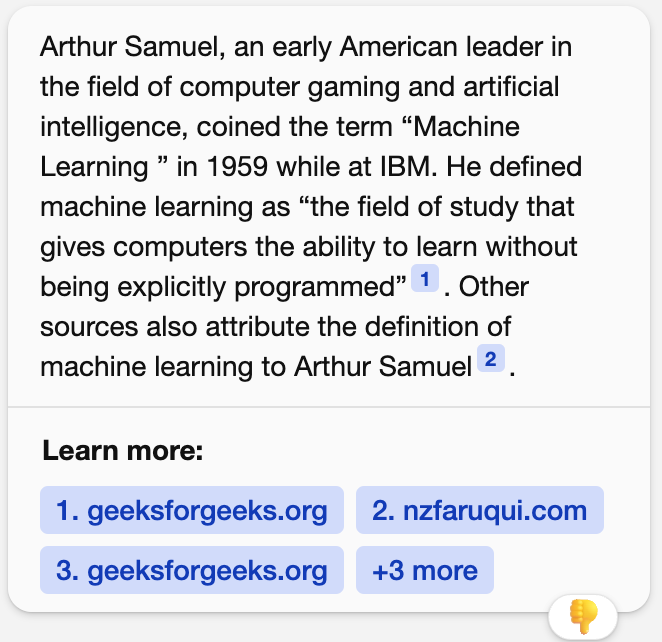
\includegraphics[width = 0.6\textwidth]{../assets/arthur-samuel-according-to-bing.png}
\end{figure}

\end{frame}


%%%%%NOTE%%%%%
\note{
\scriptsize \singlespacing

\begin{wideitemize}
\item xxxx
\end{wideitemize}

}



%-------------------------------------------------------------------------------%
\begin{frame}{What is machine learning?}

\begin{figure}
\centering
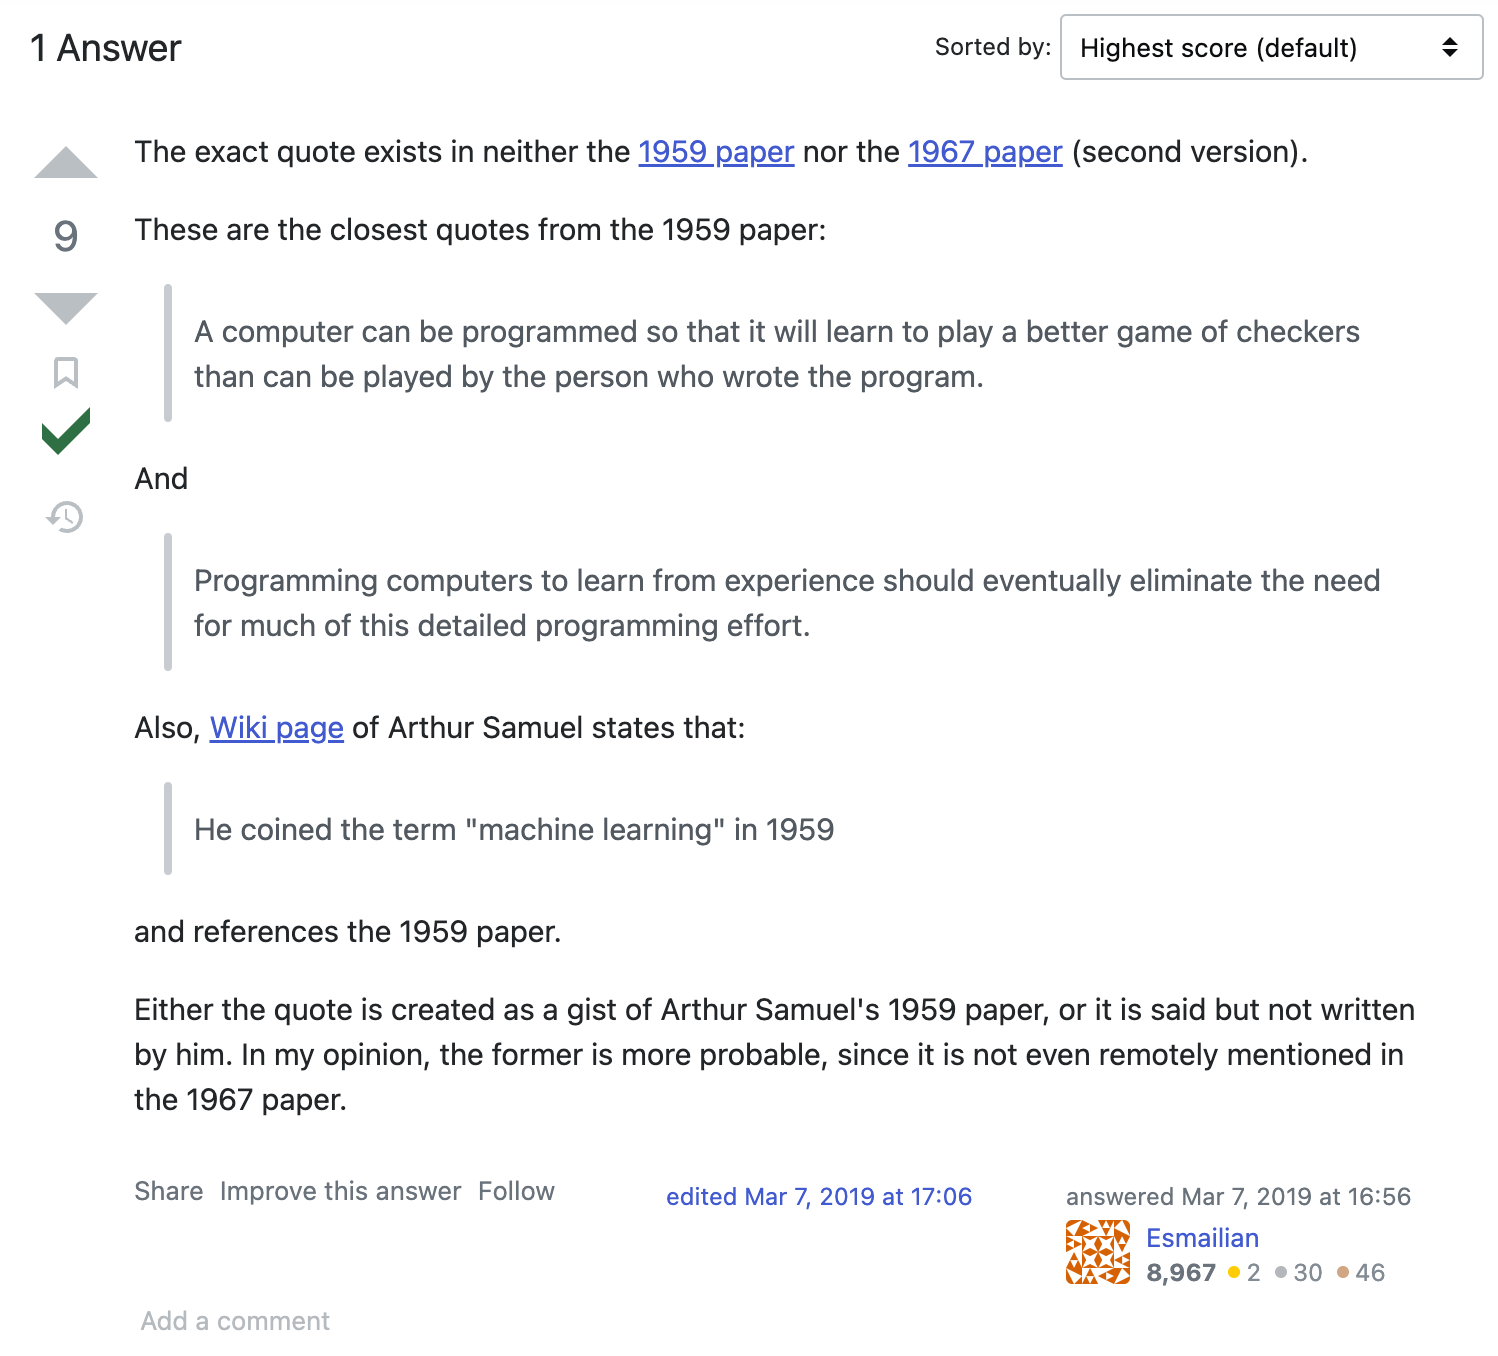
\includegraphics[width = 0.8\textwidth]{../assets/samuel-refute-stackexchange.png}
\end{figure}

\url{https://datascience.stackexchange.com/questions/37078/source-of-arthur-samuels-definition-of-machine-learning}

\end{frame}


%%%%%NOTE%%%%%
\note{
\scriptsize \singlespacing

\begin{wideitemize}
\item xxxx
\end{wideitemize}

}



%-------------------------------------------------------------------------------%

\begin{frame}{What is machine learning?}

\begin{figure}
\centering
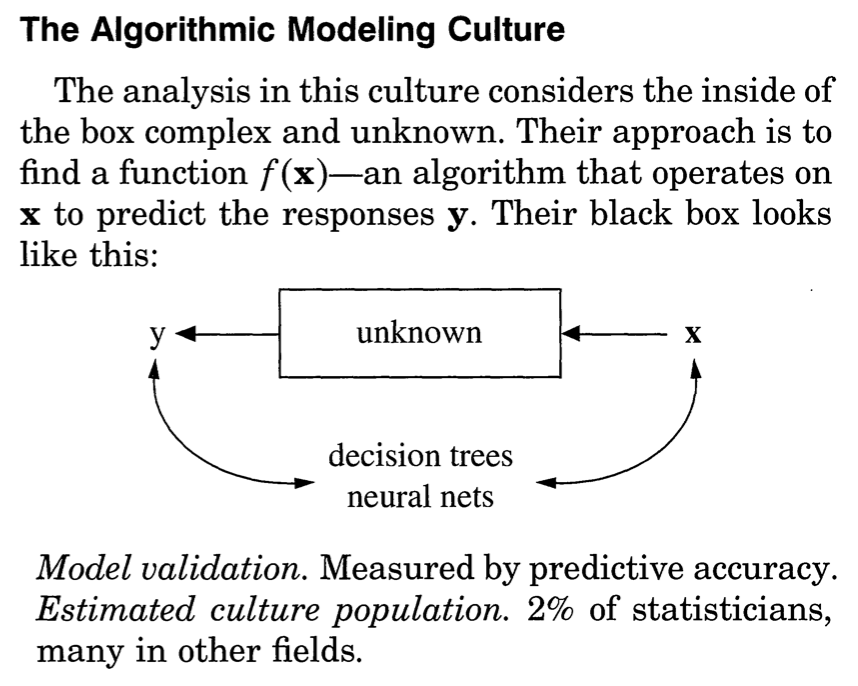
\includegraphics{../assets/breiman_2001AM-culture.png}
\end{figure}


\hfill \cite{breiman2001statistical}

\end{frame}


%%%%%NOTE%%%%%
\note{
\scriptsize \singlespacing

\begin{wideitemize}
\item xxxx
\end{wideitemize}

}



%-------------------------------------------------------------------------------%
\begin{frame}{What is machine learning?}

\begin{quote}
The traditional approach in econometrics \dots is to specify a target, an estimand, that is a functional of a joint distribution of the data.
$$
\vdots
$$
In contrast, in the ML literature, the focus is typically on developing algorithms \dots The goal for the algorithms is typically to make predictions about some variables given others or to classify units on the basis of limited information, for example, to classify handwritten digits on the basis of pixel values.
\end{quote}

\hfill \cite{athey2019machine}

\end{frame}


%%%%%NOTE%%%%%
\note{
\scriptsize \singlespacing

\begin{wideitemize}
\item xxxx
\end{wideitemize}

}



%-------------------------------------------------------------------------------%
\begin{frame}{What is machine learning?}

In the context of this class:\pause

\begin{wideitemize}
\item A culture/perspective, \pause of a research community that has developed a set of tools to tackle some common objectives, \pause which will inform how we think about framing what our research problems are, and how we go about addressing these problems. 
\end{wideitemize}

\end{frame}


%%%%%NOTE%%%%%
\note{
\scriptsize \singlespacing

\begin{wideitemize}
\item xxxx
\end{wideitemize}

}



%-------------------------------------------------------------------------------%
\begin{frame}{Some common tasks we might address with ML methods}
\pause
\begin{wideitemize}
\item Prediction for the next observation \pause
\begin{itemize}
\item Given some data $(Y_1, \X_1), \dots, (Y_N, \X_N)$, and potentially $X_{N+1}$, formulate a method to predict $\hat{Y}_{N+1}$, to minimize
\[
\left(Y_{N+1} - \hat{Y}_{N+1}\right)^2
\]
\end{itemize}
\pause
\item Conditional means estimation \pause (often in the form of augmented regression)\pause
\begin{itemize}
\item Estimate $\hat g(x)$, 
\[
g(x) = \E[Y | \X_i = x]
\]\pause
\item Is this different from the prediction problem? \pause
\item Do we have a lot of covariates? We may want to regularize, select a subset of covariates. \pause
\item Do we think the mean is not linear in covariates, and we would like to allow it to take a flexible form? 
\end{itemize}
\end{wideitemize}

\end{frame}


%%%%%NOTE%%%%%
\note{
\scriptsize \singlespacing

\begin{wideitemize}
\item xxxx
\end{wideitemize}

}

%-------------------------------------------------------------------------------%
\begin{frame}{Some common tasks we might address with ML methods}
\pause
\begin{wideitemize}
\item Supervised classification \pause
\item Unsupervised classification \pause
\item What should we do next?
\end{wideitemize}

\end{frame}


%%%%%NOTE%%%%%
\note{
\scriptsize \singlespacing

\begin{wideitemize}
\item xxxx
\end{wideitemize}

}

%-------------------------------------------------------------------------------%
\begin{transitionframe}
\centering

\LARGE \textcolor{white}{What are we actually asking from the data, and where can we find connections between machine learning and causal inference?}

\end{transitionframe}
%-------------------------------------------------------------------------------%
\begin{frame}{ML in CI}

\begin{wideitemize}
\item Estimating average treatment effects. \\ \pause
\begin{align*}
\mu(w,x) & = \E[Y_i |W_i = w, \X_i = x]\\
e(x) & = \E[W_i | \X_i = x]
\end{align*}\pause
\begin{align*}
    \onslide<3->{\tau &= \E\left[\mu(1,\X_i) - \mu(0,\X_i) \right] \\}
    \onslide<4->{ & = \E\left[\frac{Y_i W_i}{e(\X_i)} - \frac{Y_i (1-W_i) }{1 - e(\X_i)}\right] \\}
    \onslide<5>{ & = \E\left[ \frac{\left(Y_i - \mu(1,\X_i)\right)  W_i}{e(\X_i)} - \frac{\left(Y_i - \mu(0,\X_i)\right) (1-W_i) }{1 - e(\X_i)}\right] \\}
   \onslide<5>{ & \qquad \qquad  + \E\left[\mu(1,\X_i) - \mu(0,\X_i) \right]}
\end{align*}
\end{wideitemize}

\end{frame}


%%%%%NOTE%%%%%
\note{
\scriptsize \singlespacing

\begin{wideitemize}
\item xxxx
\end{wideitemize}

}

%-------------------------------------------------------------------------------%
\begin{frame}{ML in CI}

\begin{wideitemize}
\item Many of the tools we use for estimating conditional means can be used for estimating conditional average treatment effects; but may need to account for optimizing for $\tau$ rather than $\mu(\cdot)$ in e.g., parameter selection. 
\end{wideitemize}

\end{frame}


%%%%%NOTE%%%%%
\note{
\scriptsize \singlespacing

\begin{wideitemize}
\item xxxx
\end{wideitemize}

}

%-------------------------------------------------------------------------------%
\begin{frame}{ML in CI}

\begin{wideitemize}
\item In particular, this form of the estimator will come back when we read \cite{chernozhukov2018double, schuler2017targeted}:
\begin{align*}
      & = \E\left[ \frac{\left(Y_i - \mu(1,\X_i)\right)  W_i}{e(\X_i)} - \frac{\left(Y_i - \mu(0,\X_i)\right) (1-W_i) }{1 - e(\X_i)}\right] \\
     & \qquad \qquad  + \E\left[\mu(1,\X_i) - \mu(0,\X_i) \right]
\end{align*}\pause
\pause
\item We may want to estimate $\mu(w,x)$ and $e(x)$ to get better estimates of $\hat \tau$, but we don't necessarily care about how ``good'' our estimates of these parameters are. \pause
\begin{itemize}
\item[$\rightarrow$] ``nuisance'' parameters
\end{itemize}
\item We can use cross-fitting and orthogonalization to get estimates of $\mu(w,x)$ and $e(x)$ that will result in an estimator that has really nice properties: \textbf{double robustness}. 
\end{wideitemize}

\end{frame}


%%%%%NOTE%%%%%
\note{
\scriptsize \singlespacing

\begin{wideitemize}
\item xxxx
\end{wideitemize}

}

%-------------------------------------------------------------------------------%
\begin{frame}{Experimental design}

\begin{wideitemize}
\item Reinforcement learning more broadly: what action to take to optimize an objective. \pause (e.g., AlphaGo)\pause
\begin{itemize}
\item Multi-armed bandits: exploration/exploitation tradeoff. \pause Experiments addressing a broader range of objectives. \pause
\item (if time: discuss applications)
\end{itemize}

\end{wideitemize}

\end{frame}


%%%%%NOTE%%%%%
\note{
\scriptsize \singlespacing

\begin{wideitemize}
\item xxxx
\end{wideitemize}

}

%-------------------------------------------------------------------------------%
\begin{frame}{Some additional definitions}

\begin{wideitemize}
\item Cross-validation (many variants), cross-fitting \pause
\item Bootstrapping, bagging, sample splitting \pause (we'll get to these next week)\pause
\item Boosting \pause
\item We'll talk about some methods/tools: penalized regression, trees/forests, policy learning, reinforcement learning\pause, but there are a lot of approaches we won't get into (neural nets, support vector machines, many tools for classification problems, language tools) \pause and we will talk about some high-level approaches that can combine/be applied with multiple machine learning estimating techniques (doubly robust estimation, conformal inference). 
\end{wideitemize}

\end{frame}


%%%%%NOTE%%%%%
\note{
\scriptsize \singlespacing

\begin{wideitemize}
\item xxxx
\end{wideitemize}

}

%-------------------------------------------------------------------------------%
\backupbegin
%-------------------------------------------------------------------------------%

\begin{frame}[allowframebreaks]{References}
    \bibliographystyle{apalike}
    \bibliography{../assets/PLSC40601}
\end{frame}
%-------------------------------------------------------------------------------%
\backupend
\end{document}
%
%-------------------------------------------------------------------------------%

%%% [[TEMPLATE]] %%%
\begin{frame}{Frametitle}

\begin{wideitemize}
\item xxx
\end{wideitemize}

\end{frame}


%%%%%NOTE%%%%%
\note{
\scriptsize \singlespacing

\begin{wideitemize}
\item xxxx
\end{wideitemize}

}

%-------------------------------------------------------------------------------%
